\documentclass[11pt, a4paper]{article}
\usepackage{amsmath, amssymb, titling}
\usepackage[margin=3cm]{geometry}

\renewcommand\maketitlehooka{\null\mbox{}\vfill}
\renewcommand\maketitlehookd{\vfill\null}
\usepackage{enumitem}
\usepackage{graphicx}
\usepackage{float}

% \usepackage{minted}
\usepackage{xcolor}

\title{Satellite Orbit Control}
\author{Almog Dubrescu\\\\ID 214254252}

\begin{document}

\maketitle

\thispagestyle{empty}
\newpage
\setcounter{page}{1}

\tableofcontents
\vfil
\listoffigures
\newpage

\section{Given}
\begin{itemize}
    \item In ECI
    \begin{align*}
        \vec{r}_{an} = \begin{pmatrix}
            5000\\8500\\???
        \end{pmatrix} [km]
        \hspace{1cm}
        \vec{v}_{an} = \begin{pmatrix}
            2.15\\-2.05\\???
        \end{pmatrix} \left[\frac{km}{sec}\right]
    \end{align*}
    \item $$ T = 7800 [sec] $$
    \item $$ m = 450 [kg] $$
    \item $$ A_{drag} = 2 [m^2]$$
    \item $$ C_D = 2.2 [-]$$
    \item $$ A_{solar} = 5 [m^2]$$
\end{itemize}
\section{Q1}
Given:
Because the ascending node position is given in ECI, $ r_{an, 3} = 0$ so: 
\begin{equation}
    \vec{r}_{an} = \begin{pmatrix}
            5000\\8500\\0
        \end{pmatrix} [km] \hspace{0.25cm} r = 9.8615 \cdot 10^3 [km]
\end{equation}
\\
From the period:
\begin{equation}
    T = \frac{2\pi}{\sqrt{\frac{\mu}{a^3}}}
    \Rightarrow
    a = \sqrt[3]{\frac{\mu T^2}{4\pi ^2}}
    \Rightarrow
    \colorbox{yellow}{$a = 8.5007 \cdot 10^3 \left[km\right]$}
\end{equation}
\\
The velocity at the ascending node is:
\begin{equation}
    v = \sqrt{2\mu \left(\frac{1}{r} - \frac{1}{2a}\right)}
    \Rightarrow
    v = 5.8266 \left[\frac{km}{sec}\right] 
\end{equation}
\begin{equation}
    v = \sqrt{2.15^2 + 2.05^2 + v_{an, 3}^2} 
    \Rightarrow
    v_{an, 3} = \pm 5.0124 \left[\frac{km}{sec}\right] 
\end{equation}
Find the angular momentum in order to find the ascending node line:
\begin{equation}
    \vec{h} = \vec{r} \times \vec{v} = \begin{vmatrix}
        i & j & k \\ 5000 & 8500 & 0 \\ 2.15 & -2.05 & \pm 5.0124
    \end{vmatrix} = \begin{pmatrix}
        \pm 42605.4 \\ \mp 25062 \\ -28525
    \end{pmatrix}
\end{equation}
\begin{equation}
    \vec{n} = \vec{z} \times \vec{h} = -h_y\vec{x}+h_x\vec{y} = \begin{pmatrix}
        \pm 25062 \\ \pm 42605.4 \\ 0
    \end{pmatrix}
    \hspace{0.25cm} n = 4.9430\cdot 10^4
\end{equation}
\\
The radius at the ascending node is parallel to the ascending node line which means that they have the same sign in every direction:
\begin{equation}
    v_{an, 3} = 5.0124 \left[\frac{km}{sec}\right] 
    \Rightarrow
    \vec{v}_{an} = \begin{pmatrix}
        2.15\\-2.05\\5.0124
    \end{pmatrix} \left[\frac{km}{sec}\right] 
\end{equation}
\begin{equation}
    \vec{h} = \begin{pmatrix}
        42605.4 \\ -25062 \\ -28525
    \end{pmatrix}\left[\frac{km^2}{sec}\right] \hspace{0.25cm} h = 5.7070\cdot 10^4 \left[\frac{km^2}{sec}\right]
\end{equation}
\\
The eccentricity is given by:
\begin{equation}
    \vec{e} = \frac{\vec{v}\times\vec{h}}{\mu} - \frac{\vec{r}}{r} = \begin{pmatrix}
        -0.0452 \\ -0.1723 \\ 0.0839
    \end{pmatrix}
    \hspace{0.25cm} 
    \colorbox{yellow}{$e = 0.1969$}    
\end{equation}
\\
The angle of inclination $(0^\circ\leq i \leq 180^\circ)$:
\begin{equation}
    \cos (i) = \frac{h_z}{h} = \frac{-28525}{57070}
    \Rightarrow
    \colorbox{yellow}{$i = 2.0942[rad] = 119.9888^\circ$}
\end{equation}
\\
Argument of perigee:
\begin{equation}
    \cos (\omega) = \frac{\vec{n} \cdot \vec{e}}{n\cdot e},\ \  \sin (\omega) = \sqrt{1-\cos^2(\omega)}
\end{equation}
$$\Downarrow$$
\begin{equation}
    \omega = \text{atan2}\left[\text{sign}(e_z)\cdot\sqrt{1-\left(\frac{\vec{n}\cdot\vec{e}}{n\cdot e}\right)^2}, \frac{\vec{n}\cdot\vec{e}}{n\cdot e}\right]
\end{equation}
$$\Downarrow$$
\begin{align}
\colorbox{yellow}{$\omega = 2.6270 [rad] = 150.5160^\circ$}
\end{align}
Longitude of ascending node:
\begin{equation}
    \cos(\Omega) = \frac{n_x}{n},\ \ \sin(\Omega) = \frac{n_y}{n}\Rightarrow\Omega = \text{atan2}\left(\frac{n_y}{n}, \frac{n_x}{n}\right)
\end{equation}
$$\Downarrow$$
\begin{align}
\colorbox{yellow}{$\Omega = 1.0391 [rad] = 59.5303^\circ$}
\end{align}


\newpage

\section{Q2}
In order to perform the simulation of the orbit based on the equations of motion we need to list all the forces that act on the satellite:
\begin{itemize}
    \item \textbf{\Large Equations of Motion of a Point Mass in a Central Force Field:}\\
    Vector equation of motion:
    \begin{equation}
        \ddot \vec{r} = -\frac{\mu}{r^3}\vec{r}+\vec{f}
    \end{equation}
    Where:
    \begin{itemize}
        \item $\mu = \text{G}\cdot \text{M}$
        \item $\vec{r}(t_0) = \vec{r}_0$
        \item $\dot \vec{r}(t_0) = \frac{d\vec{r}}{dt}(t_0) = \vec{v}_0$
    \end{itemize}
    The equation is based on:
    \begin{itemize}
        \item Gravitational attraction between two point masses
        \item Newton's second law
        \item Assumptions: m<<M, M is homogeneous sphere
        \item $\vec{f}$ is all the external forces 
    \end{itemize}
    \item \textbf{\Large $\vec{f}$:}
    \begin{enumerate}
        \item \textbf{\large Atmospheric Drag:}  \begin{equation}
            \vec{f}_d = -\frac{1}{2}\rho v^2K_D\vec{v}
        \end{equation}
        Where:
        \begin{itemize}
            \item $\rho$ is the atmospheric density
            \item $\displaystyle{K_D = \frac{A_{drag}\cdot C_D}{m}}$
        \end{itemize}
        \underline{Density modle}:
        \begin{equation}
            \rho(h) = \rho_b\cdot e^{\frac{h-h_b}{H}}
        \end{equation}
        Where:
        \begin{itemize}
            \item H is the Scale Height
            \item $\rho_b$ is the density at the bottom of $h_b$ height layer
            \item $h_b$ is the base height
        \end{itemize}
        \item \textbf{\large Earth Oblateness ($J_2$ term):}\\
        First order perturbation acceleration:
        \begin{equation}
        \begin{cases}
            f_r &=\displaystyle -\frac{3}{2}\frac{\mu}{r^2}J_2\left(\frac{R_e}{r}\right)^2\left(1-3\sin^2(i)\sin^2(\theta^*)\right)\\
            f_\theta &=\displaystyle -3\frac{\mu}{r^2}J_2\left(\frac{R_e}{r}\right)^2\sin^2(i)\sin(\theta^*)\cos(\theta^*)\\
            f_h &=\displaystyle -3\frac{\mu}{r^2}J_2\left(\frac{R_e}{r}\right)^2\sin(i)\cos(i)\sin(\theta^*)
        \end{cases}
        \end{equation}
        \newpage
        Where:
        \begin{itemize}
            \item $J_2 = 0.0010826$ 
            \item $R_e$ is the earth radius
            \item $\theta^* = \theta+\omega$
            \item $\theta$ is the true anomaly
        \end{itemize}
        And in ECI coordinate system:
        \begin{equation}
        \begin{cases}
            f_x &=\displaystyle  -\frac{3}{2}\frac{\mu\cdot x}{r^3}J_2\left(\frac{R_e}{r}\right)^2\left(5\frac{z^2}{r^2}-1\right)\\
            f_y &=\displaystyle -\frac{3}{2}\frac{\mu\cdot y}{r^3}J_2\left(\frac{R_e}{r}\right)^2\left(5\frac{z^2}{r^2}-1\right)\\
            f_z &=\displaystyle -\frac{3}{2}\frac{\mu\cdot z}{r^3}J_2\left(\frac{R_e}{r}\right)^2\left(5\frac{z^2}{r^2}-3\right)
        \end{cases}
        \end{equation}
        \item \textbf{\large Solar Radiation Pressure:}\\
        The solar radiation acceleration is:
        \begin{equation}
            \vec{f}_s = -(1+\varepsilon)\frac{G_s}{c}\frac{A_{solar}}{m}\hat{r}_{sun}
        \end{equation}
        Where:
        \begin{itemize}
            \item $\varepsilon$ is the reflectivity coefficient $\in[0,1]$ (in our case $\varepsilon = 1$)
            \item $G_s = 1358 \left[\frac{W}{m^2}\right]$ 
            \item c is the speed of light $\left(2.9979\cdot10^8\left[\frac{m}{s}\right]\right)$
        \end{itemize}
        The unit vector from Earh to the sun:
        \begin{equation}
            \hat{r}_s = \begin{pmatrix}
                \cos(\delta)\cos(RA)\\
                \cos(\delta)\sin(RA)\\
                \sin(\delta)
            \end{pmatrix}
        \end{equation}
        Where:
        \begin{itemize}
            \item $RA = 0.98563(N-80)^\circ$
            \item $\sin(\delta) = 0.39795\cdot\cos\left(0.98563(N-173)^\circ\right)$
            \item N = datenum(['our date']) - datenum(['1-Jan']) + 1 (in MatLab)
        \end{itemize}
        \newpage
        \underline{Shadow Model}:
        \begin{figure}[H]
        \begin{center}
        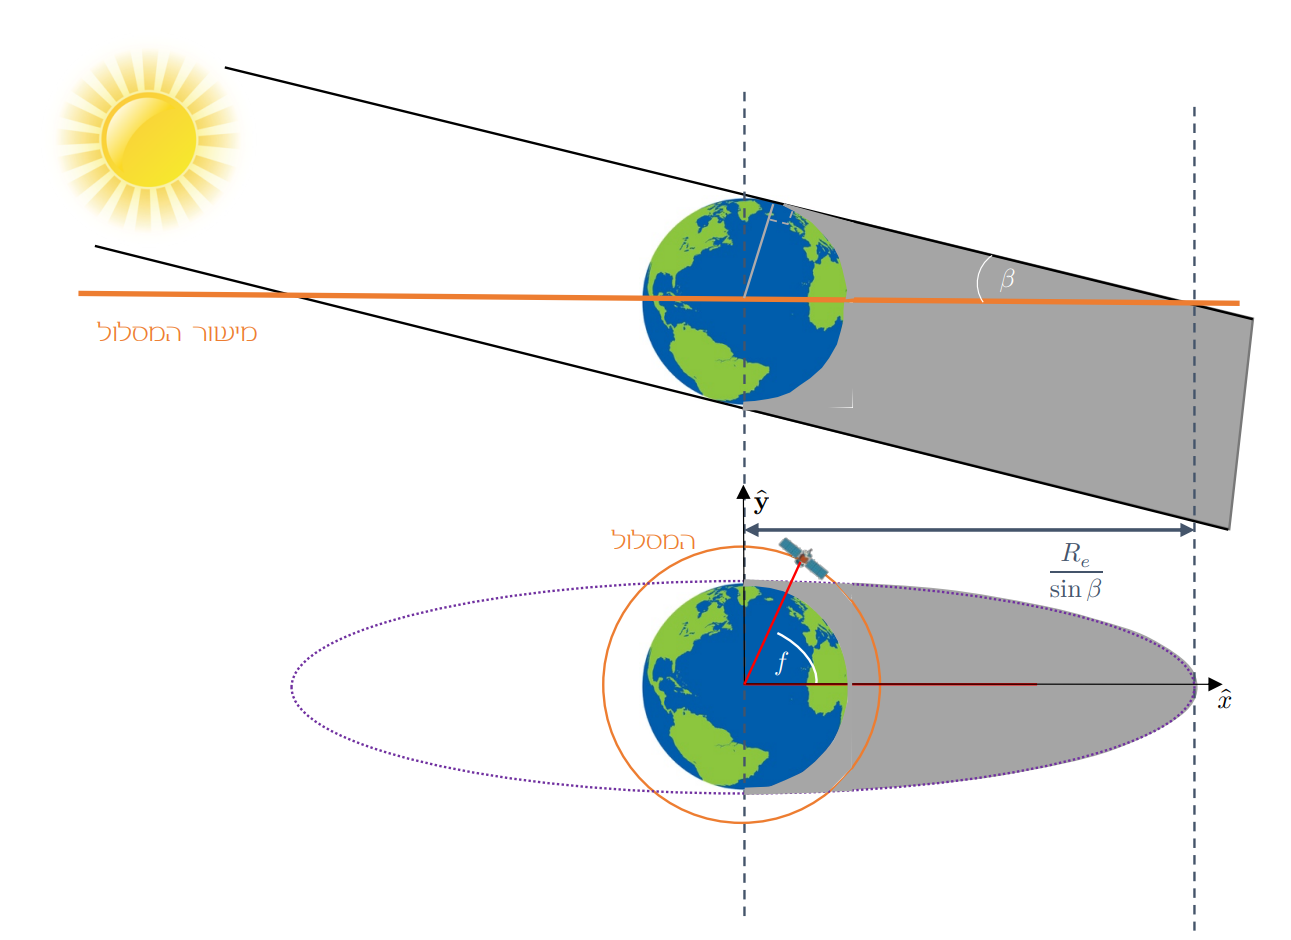
\includegraphics[width=.8\textwidth]{images/shadow model.png}
        \caption{shadow model \cite{SM_Tutorial_10}}
        \end{center}
        \end{figure}
        Assuming a cylindrical shadow, there are two condition for the satellite to be in the earth's shadow:
        \begin{enumerate}
            \item $\vec{r}\cdot\vec{r}_s < 0$
            \item $r\cdot\sin\left(\arccos\left(\vec{r}_s\cdot\vec{r}\right)\right) < Re$
        \end{enumerate}

    \end{enumerate}
\end{itemize}
\textbf{\Large The Simulation Results:}
\begin{figure}[H]
    \begin{center}
    \includegraphics[width=.8\textwidth]{images/grap1.png}
    \caption{xyz 3D plot of orbit}
    \end{center}
\end{figure}
\begin{figure}[H]
    \begin{center}
    \includegraphics[width=.8\textwidth]{images/grap1.1.png}
    \caption{xyz 3D plot of orbit - zoom}
    \end{center}
\end{figure}
\noindent We can see that because of the perturbations, the orbit does not close and overlap a bit.
\begin{figure}[H]
    \begin{center}
    \includegraphics[width=.8\textwidth]{images/grap2.png}
    \caption{orbit elements}
    \end{center}
\end{figure}
We can see that the \emph{a, e, i, $\omega$} doesn't really change after one period, but the \emph{Longitude of the ascenging node} groth monotonous over the period.
\newpage

\section{Q3}
A Tangential positive velocity change of $10\left[\frac{m}{sec}\right]$ was applied at the perigee. The new orbital elements immediately after teh pulse are:
\begin{equation}
    \Delta\vec{v} = \begin{pmatrix}
        \Delta v_t \\
        \Delta v_n \\
        \Delta v_h
    \end{pmatrix}
    =
    \begin{pmatrix}
        10 \\ 0 \\ 0
    \end{pmatrix}
    \left[\frac{m}{sec}\right]
\end{equation}
For small velocity change we get:
\begin{equation}
    \begin{pmatrix}
        \Delta a\\
        \Delta e\\
        \Delta i\\
        \Delta \Omega\\
        \Delta \omega\\
        \Delta M
    \end{pmatrix}
    = \begin{pmatrix}\
        \frac{2a}{rv}\left(2a-r\right) & 0 & 0 \\
        \frac{2}{v}\left(e+\cos\left(\theta\right)\right) & \frac{r}{av}\sin\left(\theta\right) & 0 \\
        0 & 0 & \frac{r}{h}\cos\left(\theta^*\right) \\
        0 & 0 & \frac{r}{h}\frac{\sin\left(\theta^*\right)}{\sin\left(i\right)} \\
        \frac{2}{ev}\sin\left(\theta^*\right) & -\frac{1}{ev}\left(2e+\frac{r}{a}\right)\cos\left(\theta\right) &  -\frac{r}{h}\frac{\sin\left(\theta^*\right)\cos\left(i\right)}{\sin\left(i\right)} \\
        -\frac{2\sqrt{1-e^2}}{ev}\left(1+\frac{e^2r}{p}\right)\sin\left(\theta\right) & \frac{r\sqrt{1-e^2}}{eva}\cos\left(\theta\right) & 0

    \end{pmatrix}
    \begin{pmatrix}
        \Delta v_t \\
        \Delta v_n \\
        \Delta v_h
    \end{pmatrix}
\end{equation}
multipling in MatLab we get:
\begin{equation}
    \begin{pmatrix}
        \Delta a\\
        \Delta e\\
        \Delta i\\
        \Delta \Omega\\
        \Delta \omega\\
        \Delta M
    \end{pmatrix}
    =
    \begin{pmatrix}
        3.0311\cdot10^4 \\
        2.8635 \\ 
        0 \\ 
        0 \\
        5.9793 \\ 
        0
    \end{pmatrix}
\end{equation}
$$\Downarrow$$
\begin{equation}
\begin{matrix}
    \colorbox{yellow}{$a = 3.8812\cdot10^4$}\\
    \colorbox{yellow}{$e = 3.0604$}\\
    \colorbox{yellow}{$i = 2.0942[rad] = 119.9888^\circ$}\\
    \colorbox{yellow}{$\Omega = 1.0391 [rad] = 59.5303^\circ$}\\
    \colorbox{yellow}{$\omega = 8.6063 [rad] = 133.1047^\circ$}
\end{matrix}
\end{equation}

\newpage
\bibliographystyle{ieeetr}
\bibliography{references}

\end{document}
